\documentclass{beamer}
\usepackage[utf8]{inputenc}
\usepackage[T1]{fontenc}
\usepackage{graphicx}
\usepackage{tcolorbox}
\usepackage{hyperref}
\hypersetup{
    colorlinks=true,
    linkcolor=white,
    urlcolor=cyan,
    urlbordercolor=cyan,
}
\graphicspath{ {./images/} }

\usetheme{Arguelles}

\title{Tutorial 1}
\subtitle{CS3241 Computer Graphics (AY22/23)}
\date{\today}
\author{Wong Pei Xian}
\institute[]{\email{e0389023@u.nus.edu}}

\begin{document}

\frame[plain]{\titlepage}

\section{Question 1}

\begin{frame}
    \frametitle{Question 1}
    To be able to display \textbf{realistic} images, our display devices need to be able to produce 
    every frequency in the visible light spectrum.
    
    \vspace*{1em}
    
    True or false? Why? What are the advantages and disadvantages?
\end{frame}

\begin{frame}
    \frametitle{Three-Color Theory}

    To be \textbf{realistic to human} \\
    $\Rightarrow$ To be compatible with 
    \textcolor{red}{human} \textcolor{blue}{visual} \textcolor{green}{system}
    (L01, slide 35)

    \begin{itemize}
        \item Rods: Monochromatic
        \item \textbf{Cones}: Color sensitive to wavelengths
        \begin{itemize}
            \item Long \textcolor{red}{$\approx$ red}
            \item Medium \textcolor{green}{$\approx$ green}
            \item Short \textcolor{blue}{$\approx$ blue}
        \end{itemize}
    \end{itemize}

    \textbf{Proportion} of the three gives us the sensation of different colors.
\end{frame}

\begin{frame}
    \frametitle{Cone sensitivity and Additive color theory}

    Single frequency = proportion of responses of each cone.

    \begin{center}
        \includegraphics[scale=0.2]{images/cone-vision.png}
    \end{center}

\end{frame}

\begin{frame}
    \frametitle{Additive Color Display}
    \framesubtitle{Pros}

    \begin{enumerate}
        \item We don't have to produce light of every wavelength in vis. light spectrum for realism
        \item We can see colors that are \textbf{NOT} on vis. light spectrum (e.g. \textcolor{purple}{\textbf{PURPLE}}).
        \begin{itemize}
            \item Visible colors are different combinations of amount of activity in RGB cones
            \item \textcolor{purple}{Purple} is not a specific wavelength but a combination of red and blue wavelengths 
            (unlike \textcolor{violet}{violet} which has its own wavelength)
        \end{itemize}
    \end{enumerate}

\end{frame}

\begin{frame}
    \frametitle{Additive Color Display}
    \framesubtitle{Cons}

    Two different RGB values can produce the same color.\\

    \begin{tcolorbox}
        Q: What's an example of this?\\

        A: There is no definitive inverse mapping of RGB to a wavelength, as it is display dependent. \\
        {\tiny \url{https://physics.stackexchange.com/questions/248139/can-two-different-rgb-color-triplets-give-the-same-color}}
    \end{tcolorbox}
    
\end{frame}

\section{Question 2}

\begin{frame}
    \frametitle{Question 2}

    Each pixel in a frame-buffer has 8 bits for each of the R, G and B channels. How many different
    colors can each pixel represent? Is this enough?

    \begin{tcolorbox}
        8 bits per channel (R, G, B): $2^{24} = \textbf{16,777,216}$ colors. 
    \end{tcolorbox}

\end{frame}

\begin{frame}
    \frametitle{32-bit color}

    In most graphical applications today, we have 4 channels:
    \begin{itemize}
        \item R
        \item G
        \item B
        \item (not included in this question) A for Alpha (transparency)
    \end{itemize}

    Hence color has 32 bits: $2^{32}$ values (can be represented with an \texttt{int})!

    On color depth: \url{https://computer.howstuffworks.com/monitor4.htm}

\end{frame}

\begin{frame}
    \frametitle{32-bit color}
    \framesubtitle{Is this enough?}

    256 shades of gray: \textbf{banding artifacts}.

    \begin{center}
        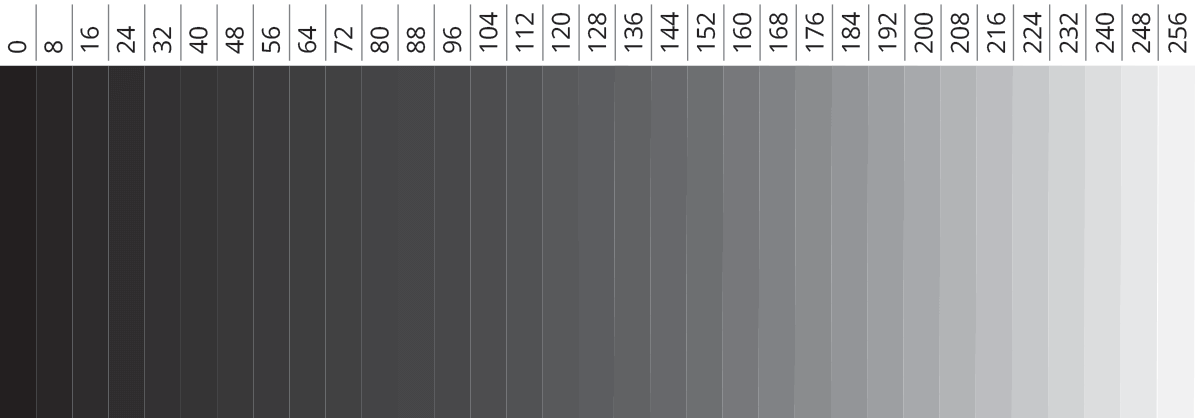
\includegraphics[scale=0.25]{greyscale-levels.png}
    \end{center}

    Use case decides if this is undesirable or not.

\end{frame}

\begin{frame}
    \frametitle{8-bit representation of color}
    On some systems, each pixel has only 8 bits (for all R, G, and B combined). 
    How would you allocate the bits to the R, G and B primaries?

    \begin{center}
        \includegraphics[scale=0.2]{cone-vision.png}
    \end{center}

\end{frame}

\begin{frame}
    \frametitle{8-bit representation of color}
    On some systems, each pixel has only 8 bits (for all R, G, and B combined). 
    How would you allocate the bits to the R, G and B primaries?

    \begin{tcolorbox}
        3:3:2 for R:G:B. Our eyes are less sensitive to changes in blue, 
        as you can see from the normalized cone response for high frequencies.
    \end{tcolorbox}

\end{frame}

\section{Question 3}

\begin{frame}
    \frametitle{Question 3}
    Referring to Lecture 1 Slide 31. If an imaginary image plane is d unit distance in front of the
    pinhole camera, what are the coordinates of the projection (on the imaginary image plane) of
    the 3D point (x, y, z)?
\end{frame}

\begin{frame}
    \frametitle{Similar triangles}

    \begin{center}
        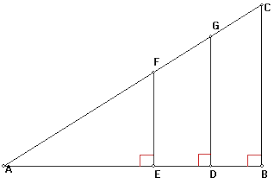
\includegraphics[scale=0.8]{similar-tris.png}
    \end{center}

    $$
    \frac{AE}{AD} = \frac{AF}{AG} = \frac{EF}{DG}
    $$

\end{frame}

\begin{frame}
    \frametitle{Perspective}

    \begin{center}
        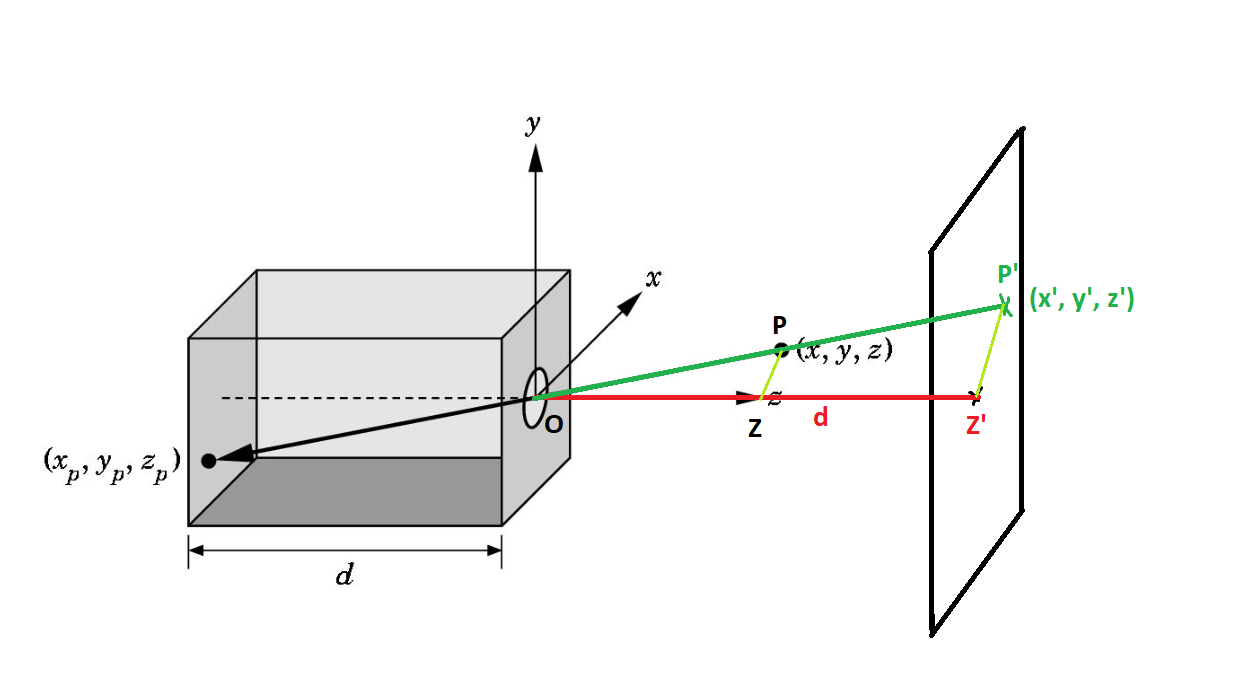
\includegraphics[scale=0.25]{q3-qn.png}
    \end{center}

    Notice that $OPZ$ and $OP'Z'$ are similar triangles as their internal angles are identical.

    $$
    \frac{x}{x'} = \frac{y}{y'} = \frac{z}{z'} \text{ and by definition } z' = d
    $$

\end{frame}

\section{Question 4}

\begin{frame}
    \frametitle{Question 4}
    Why do we need a \textbf{primitive assembly} stage in the rendering pipeline architecture?

    \vspace{1em}

    {\centering 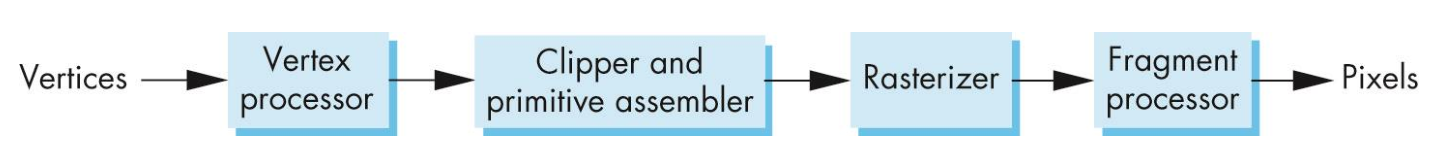
\includegraphics[scale=0.4]{simple-pipeline.png}}

    \begin{tcolorbox}
        \textbf{Primitive}: One polygonal unit
    \end{tcolorbox}
\end{frame}

\begin{frame}
    \frametitle{Primitive Assembly}
    \framesubtitle{Rendering pipeline}
    
    {\centering 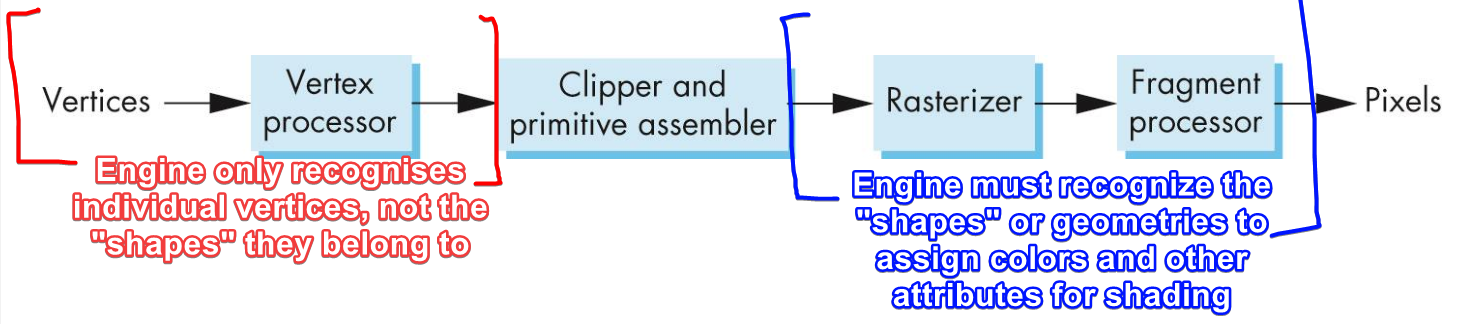
\includegraphics[scale=0.4]{simple-pipeline-annot.png}}

    {\begin{center} 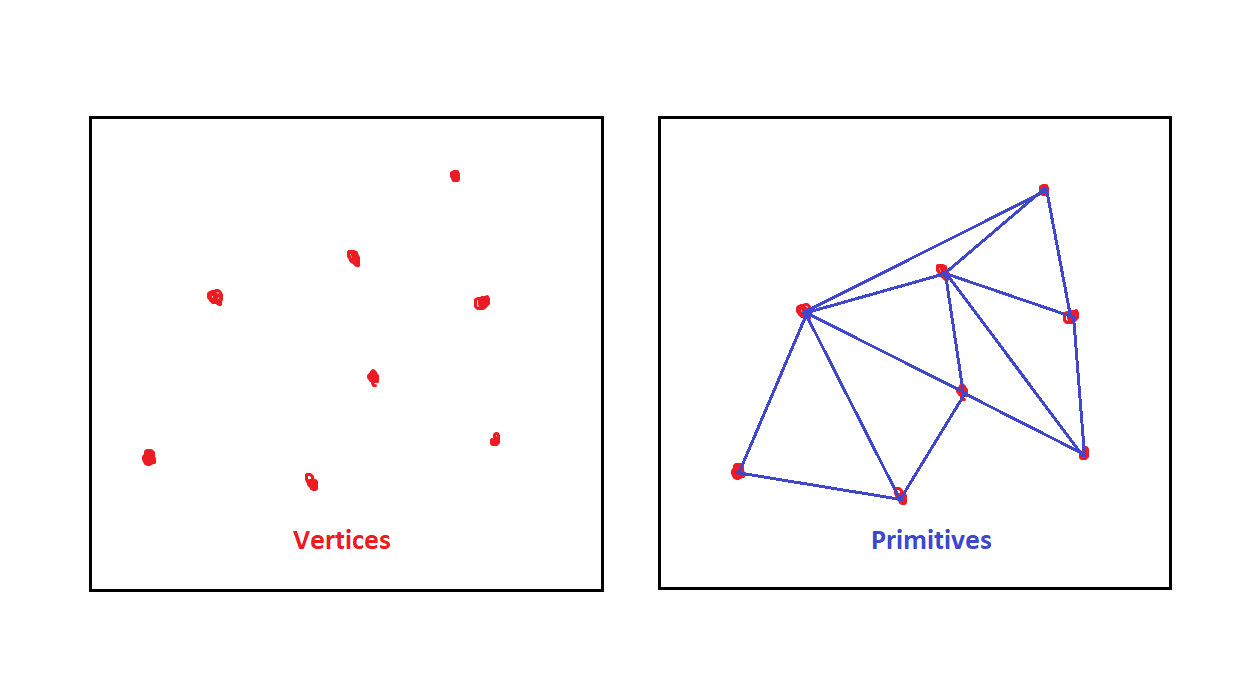
\includegraphics[scale=0.28]{q4-vert-prim.png} \end{center}}

\end{frame}

\section{Question 5}

\begin{frame}
    \frametitle{Question 5}
    What does the rasterization stage (rasterizer) do in the rendering pipeline architecture?
\end{frame}

\begin{frame}
    \frametitle{Question 5}
    Describe what it does to a triangle that is supposed to be filled, and the three vertices have
    different color. Assume smooth shading is turned on.
\end{frame}

\begin{frame}
    \frametitle{Rasterization}
    \framesubtitle{Rendering pipeline}

    (Lecture 1 Slide 40)

    Assigning colors to pixels occupied by a primitive/polygon.

    \begin{enumerate}
        \item Each vertex has an attribute.
        \item Each attribute is \textbf{interpolated} across the vertices.
    \end{enumerate}

    \vspace{1em}

    {\begin{center} 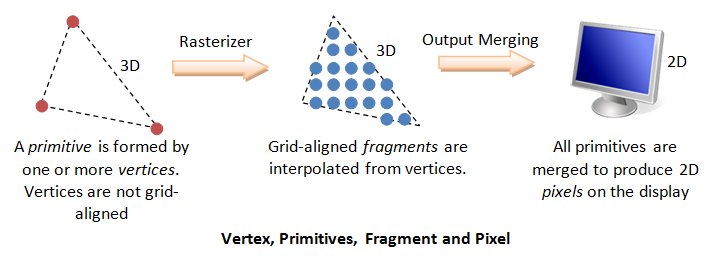
\includegraphics[scale=0.5]{q5-Graphics3D_VertexFragment.png} \end{center}}

\end{frame}

\begin{frame}
    \frametitle{Rasterization}

    Which attributes can be interpolated?
    \begin{itemize}
        \item Position
        \item Colour
        \item Normals
        \item UV coordinates
        \item Anything else that vertices may describe
    \end{itemize}

    Interpolation methods include:
    \begin{itemize}
        \item \href{https://www.scratchapixel.com/lessons/3d-basic-rendering/ray-tracing-rendering-a-triangle/barycentric-coordinates.html}{Barycentric interpolation}
        \item \href{https://en.wikipedia.org/wiki/Scanline_rendering}{Scanline algorithms (don't worry about this till week 6)}
    \end{itemize}

\end{frame}

\section{Question 6}

\begin{frame}
    \frametitle{Question 6}
    What is hidden-surface removal? When is it not necessary?
\end{frame}

\begin{frame}
    \frametitle{Hidden Surface Removal}

    After rasterization: we can have multiple fragments with the same pixel coordinates.

    \begin{center}
        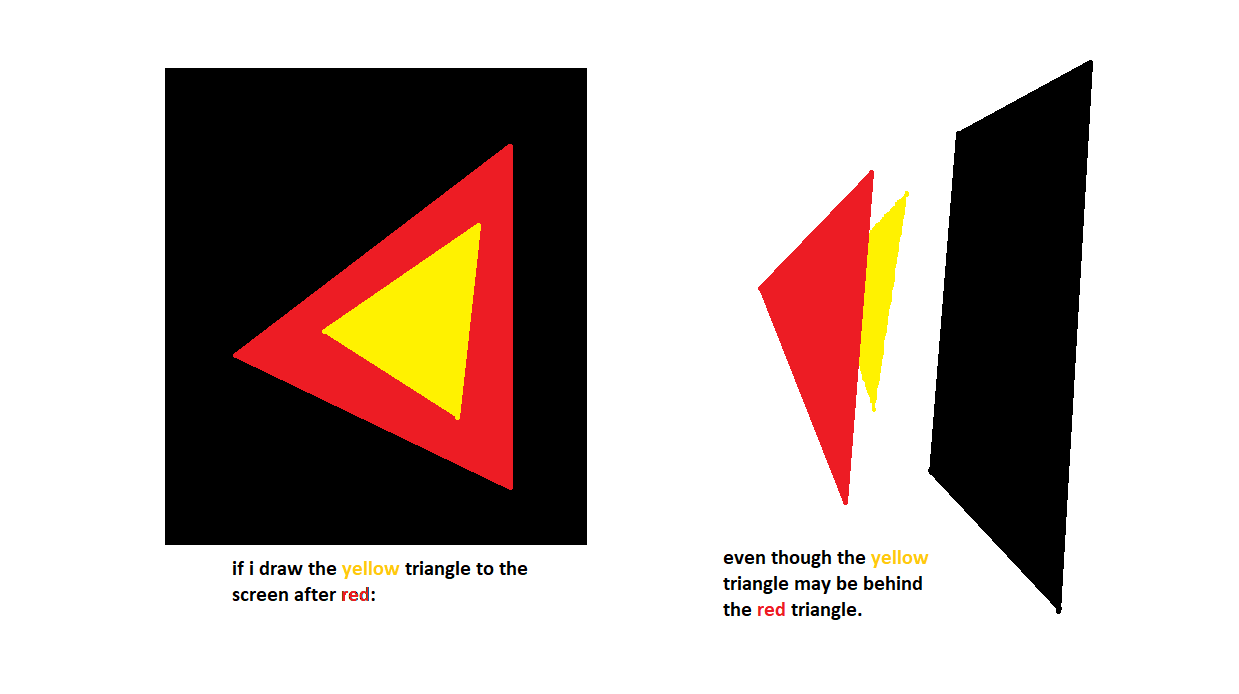
\includegraphics[scale=0.25]{q6-hsr.png}
    \end{center}

    The correct fragments to render are those that are \textbf{closest to the camera} 
    at the same pixel coordinates. 
    
    We should discard or overwrite entire hidden surfaces/fragments.

\end{frame}

\begin{frame}
    \frametitle{Hidden Surface Removal}

    Hence if
    \begin{enumerate}
        \item we have no overlapping surfaces, or
        \item we are already rendering from back to front
    \end{enumerate}
    then we don't need hidden surface removal.

    \begin{tcolorbox}
        HSR also has the added benefit of reducing rendering workload 
        (remove pixels/whole surfaces from rendering pipeline).
    \end{tcolorbox}

\end{frame}

\begin{frame}
    \frametitle{Some hidden surface removal \href{https://gabrielgambetta.com/computer-graphics-from-scratch/12-hidden-surface-removal.html}{techniques}}

    \begin{center}
        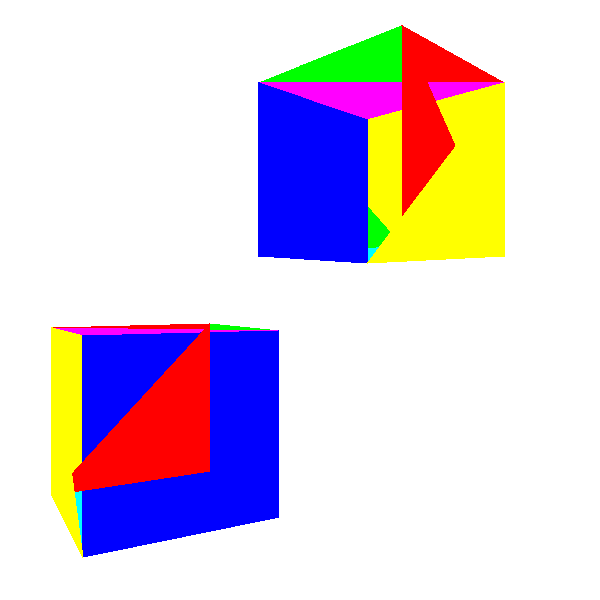
\includegraphics[scale=0.2]{hsr.png}
    \end{center}

\end{frame}

\section{Question 7}

\begin{frame}
    \frametitle{Question 7}
    Which of the two following program fragments is more efficient? Why?

    \begin{center}
        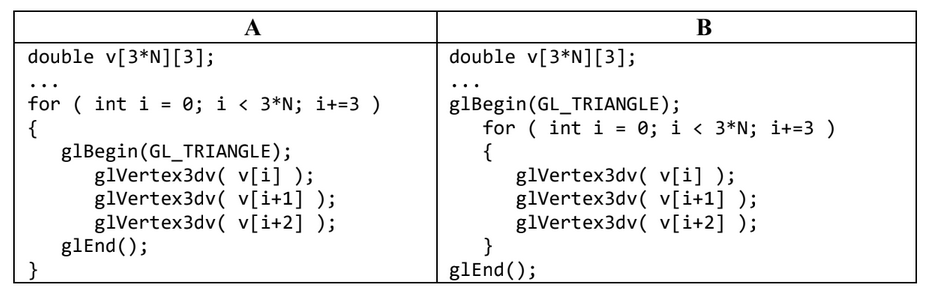
\includegraphics[scale=0.7]{q7.png}
    \end{center}

    Can the same optimization be done for the case of \texttt{GL\_POLYGON}?
\end{frame}

\begin{frame}
    \frametitle{Calls to \texttt{glBegin} and \texttt{glEnd}}

    \begin{center}
        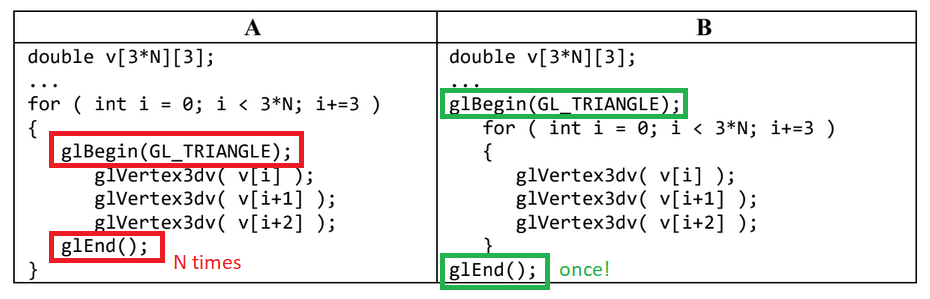
\includegraphics[scale=0.6]{q7-annot.png}
    \end{center}

    Note that OpenGL (together with mosts other graphics engines)
    is a \textbf{state machine}. Method B greatly reduces the number of state changes.

\end{frame}

\begin{frame}
    \frametitle{What about GL\_POLYGON?}

    We can't do this with GL\_POLYGON or we'll be defining one massive
    $3N$-vertex polygon.

    \begin{center}
        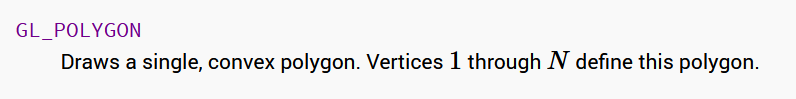
\includegraphics[scale=0.6]{gl-polygon.png}
    \end{center}

\end{frame}

\begin{frame}
    \frametitle{WebGL State Machine \href{https://webglfundamentals.org/webgl/lessons/resources/webgl-state-diagram.html}{visualizer/debugger tool}}

    \begin{center}
        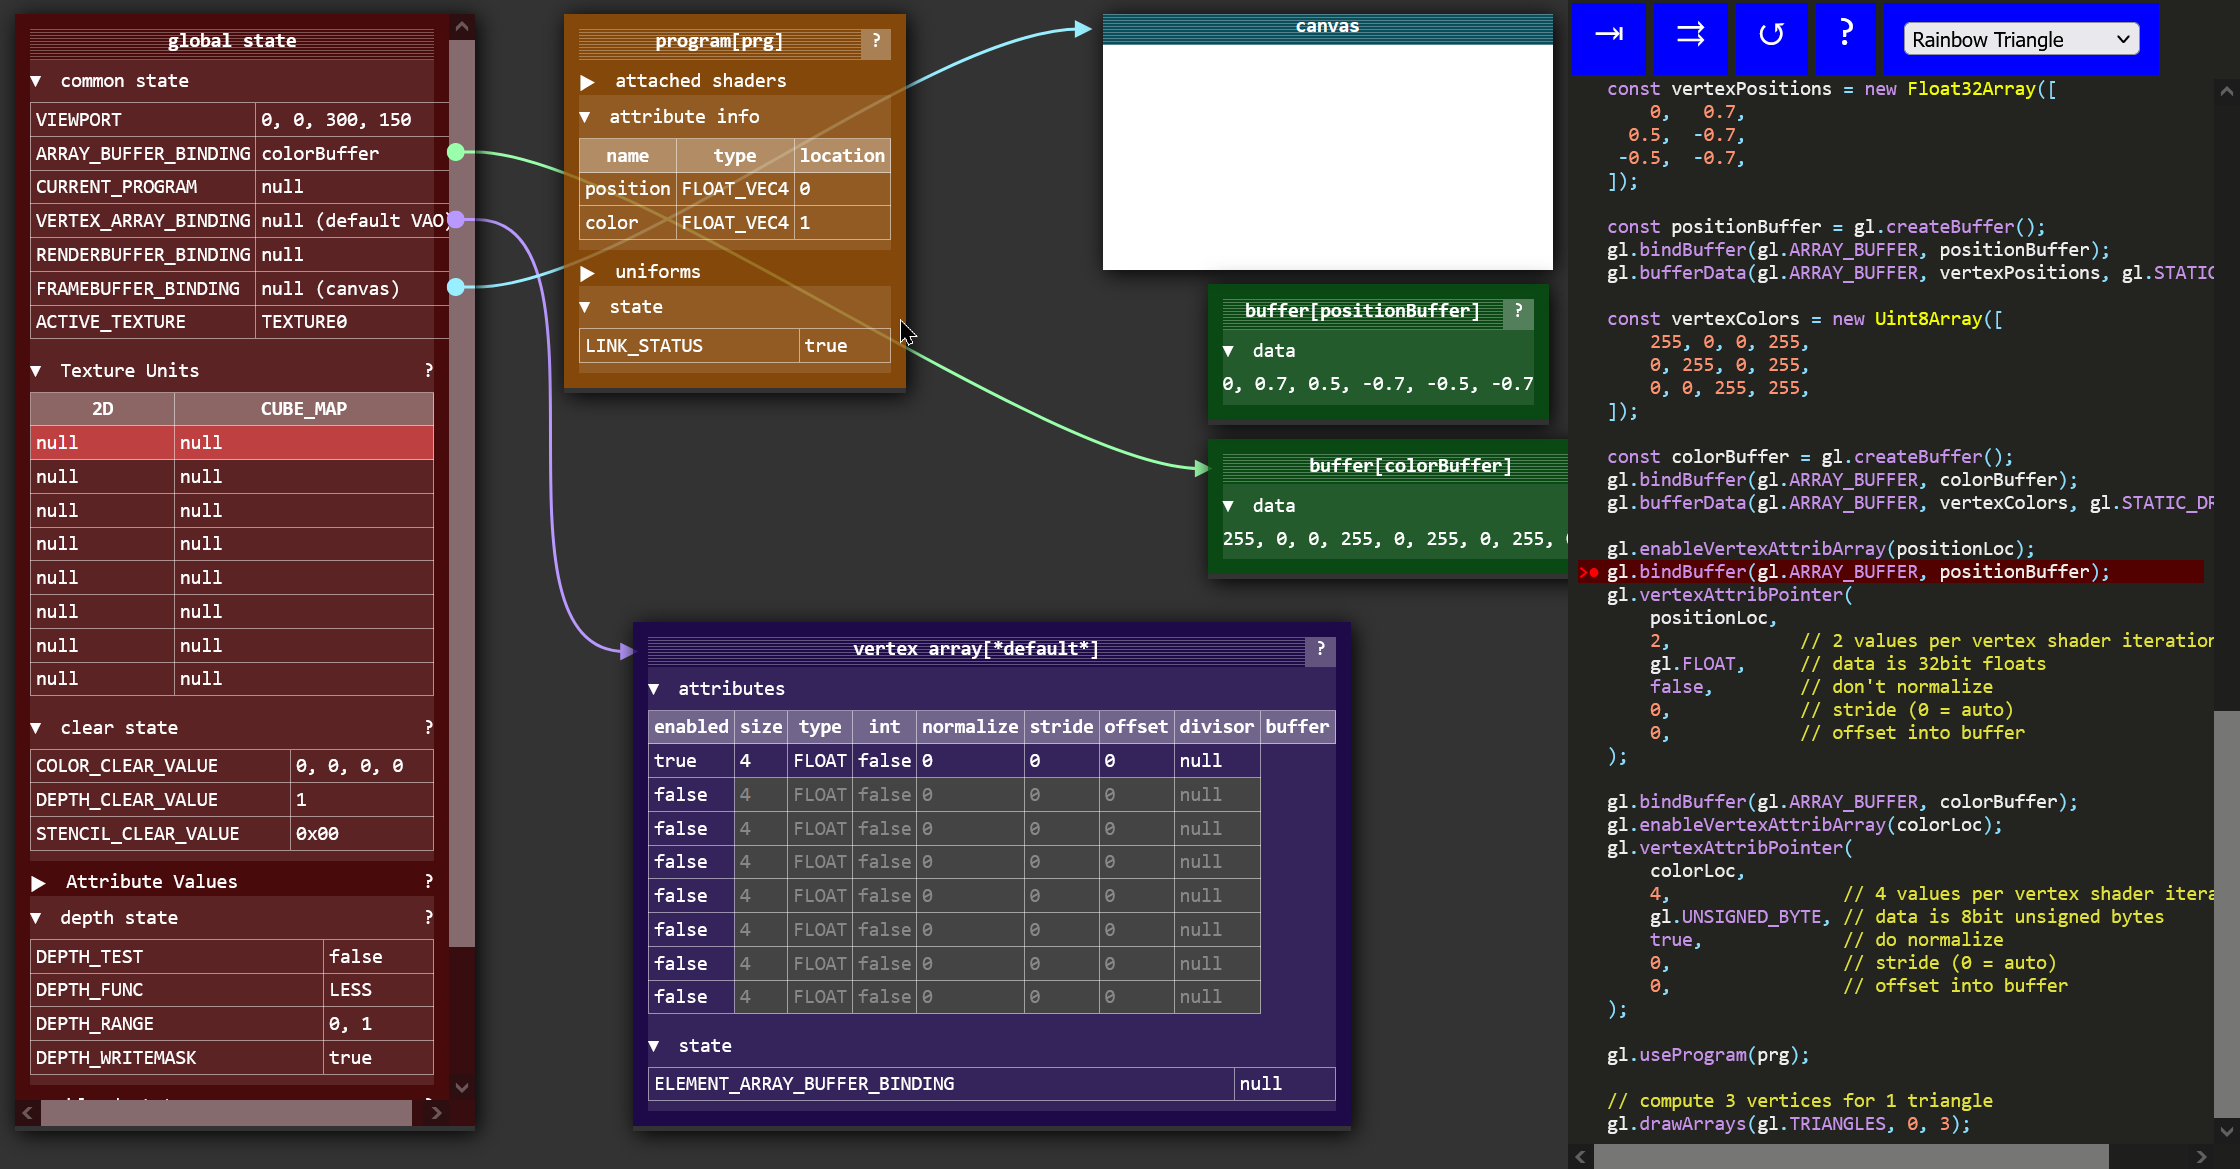
\includegraphics[scale=0.28]{webgl-fsm.png}
    \end{center}

\end{frame}

\section{Question 8}

\begin{frame}
    \frametitle{Question 8}
    OpenGL supports the GL\_TRIANGLES primitive type. Why do you think that OpenGL also
    supports GL\_TRIANGLE\_FAN and GL\_TRIANGLE\_STRIP?

    \begin{center}
        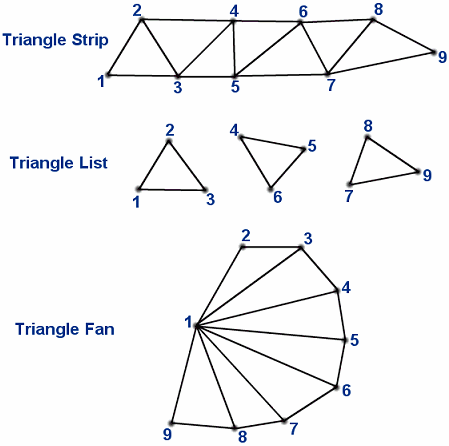
\includegraphics[scale=0.3]{tri-fan-strip.png}
    \end{center}
\end{frame}

\begin{frame}
    \frametitle{Comparison}

    \begin{center}
        \begin{tabular}{|c|c|c|}
            \hline
            Type & Vertices & Triangles\\
            \hline
            GL\_TRIANGLES & 3n & n\\
            GL\_TRIANGLE\_FAN & n + 2 & n\\
            GL\_TRIANGLE\_STRIP & n + 2 & n\\
            \hline
        \end{tabular}
    \end{center}

\end{frame}

\section{Question 9}

\begin{frame}
    \frametitle{Question 9}
    Devise a test to check whether a polygon in 3D space is planar.
\end{frame}

\begin{frame}
    \frametitle{Method from Tutorial answer}

    \begin{center}
        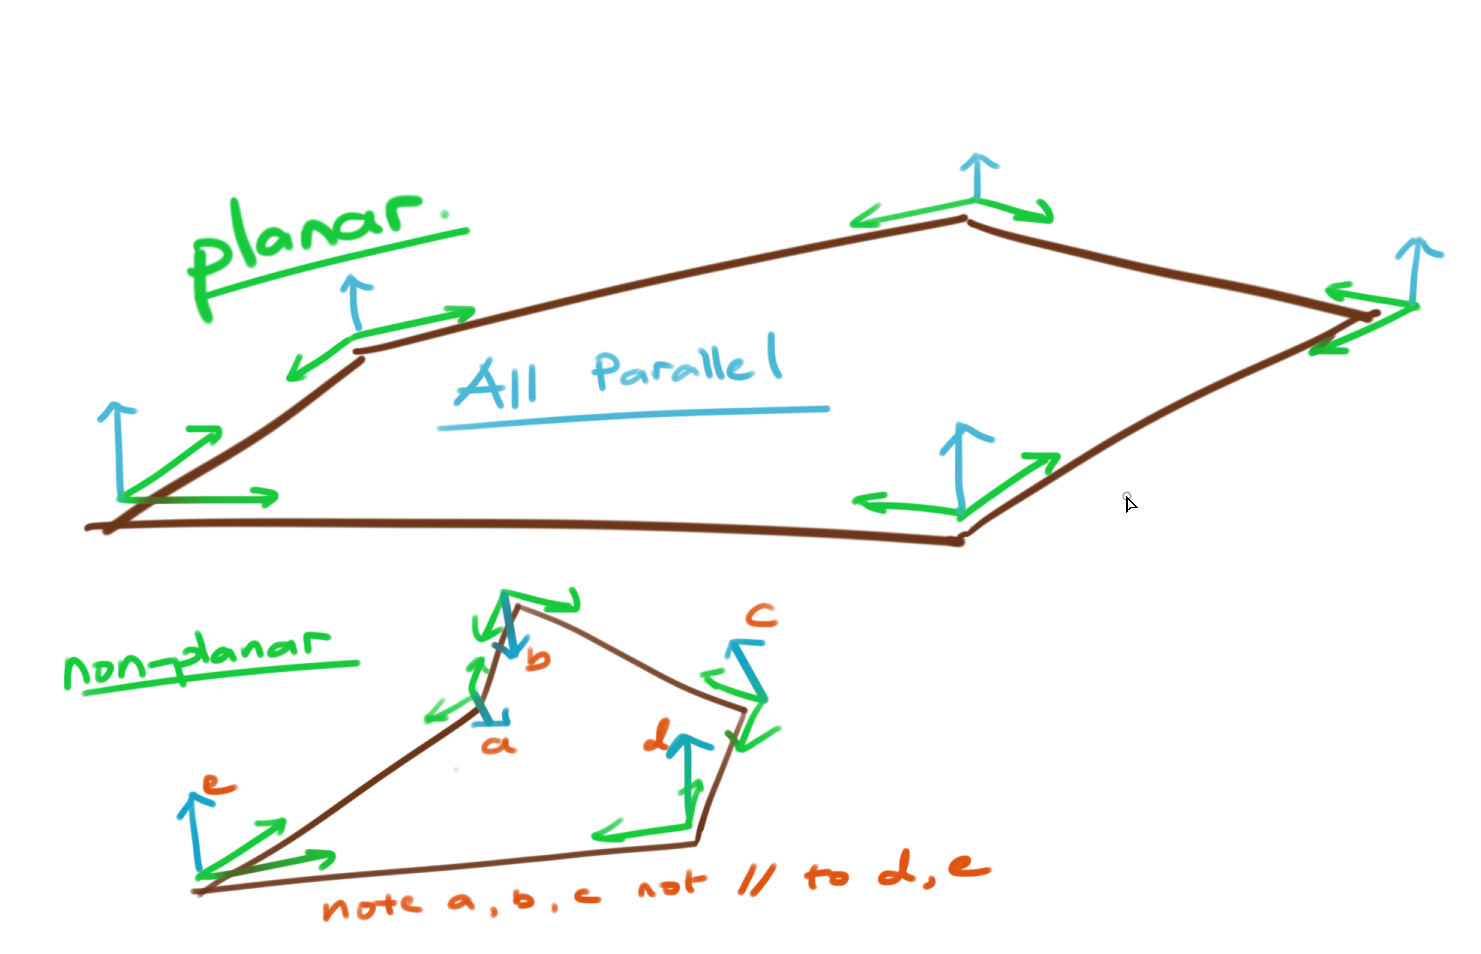
\includegraphics[scale=0.25]{planar.png}
    \end{center}

    \begin{enumerate}
        \item For each vertex, take the cross product of its two neighbouring edges.
        \item Normalize the cross product.
        \item Identify if all the cross products of each vertex are the same.
    \end{enumerate}

    \begin{tcolorbox}
        Slow because cross product computation is expensive.
    \end{tcolorbox}
    
\end{frame}

\begin{frame}
    \frametitle{Improved method}

    Note that a plane can be defined by the following equation:

    $$
    n \cdot (p - p_0) = 0
    $$

    where $n$ is the \textbf{normal of the plane}. 

    \begin{center}
        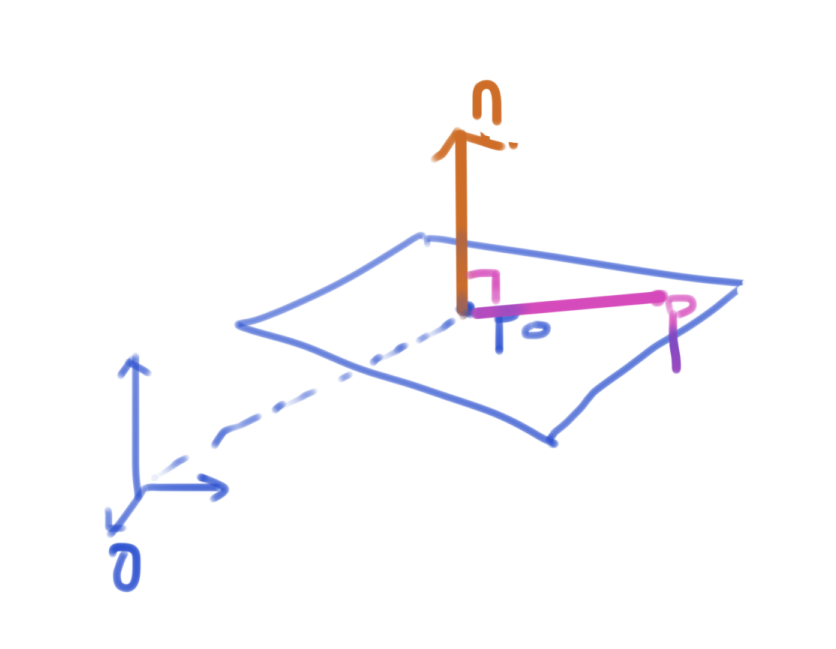
\includegraphics[scale=0.3]{plane-def.png}
    \end{center}

    This is because dot product of two vectors is zero if and only if they are perpendicular!

\end{frame}

\begin{frame}
    \frametitle{Improved method}

    Hence let's set the normal of this polygon to be $(v_1 - v_2) \times (v_3 - v_2)$.

    \begin{center}
        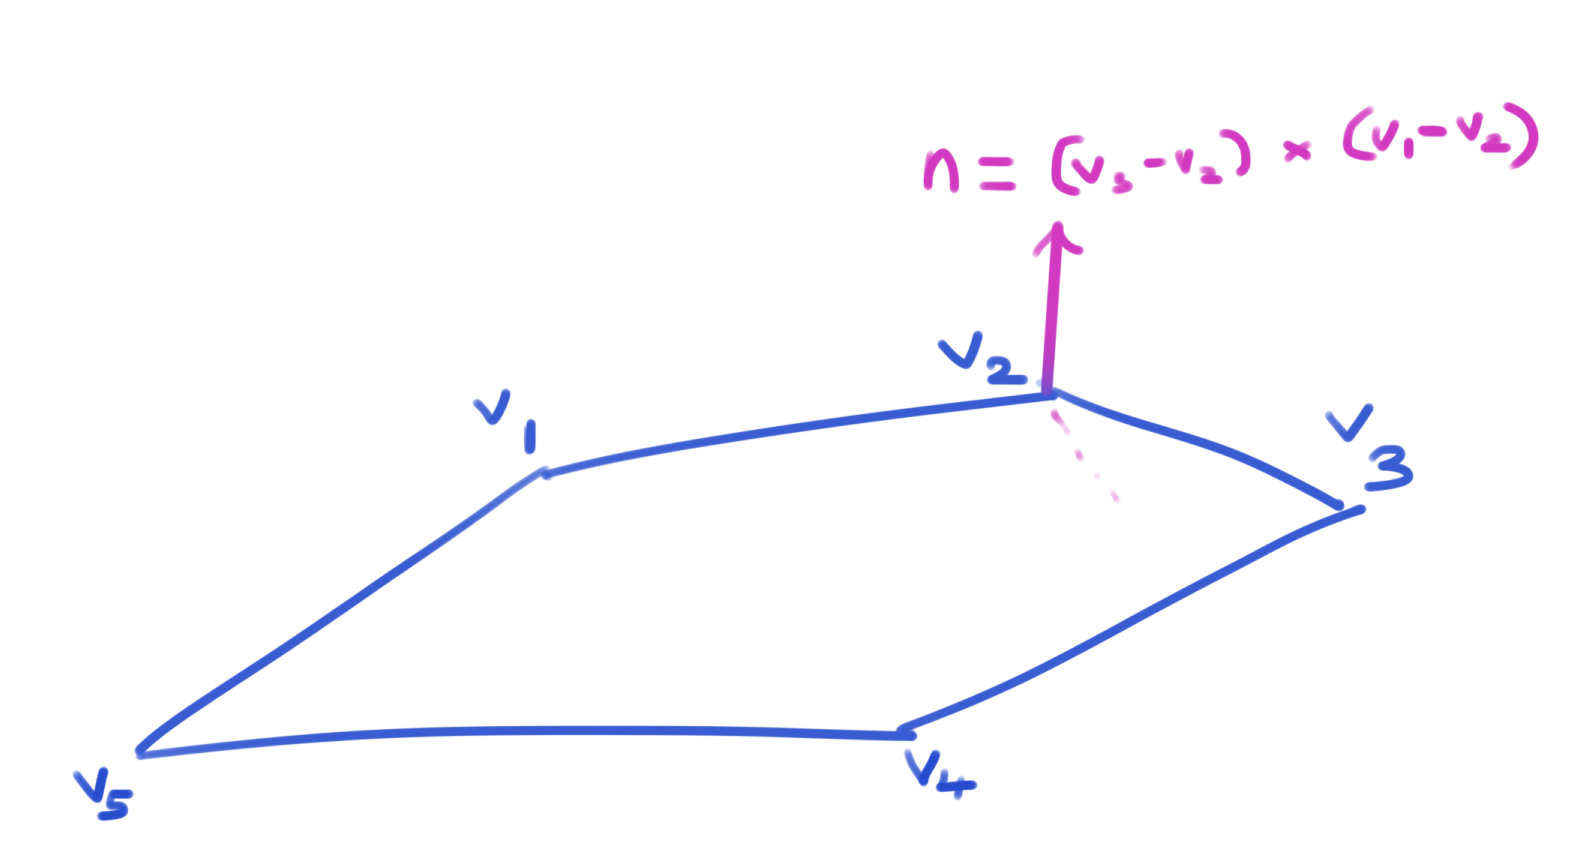
\includegraphics[scale=0.25]{planar-m2.png}
    \end{center}

\end{frame}

\begin{frame}
    \frametitle{Improved Method}

    For each of the vertices $v_i \in \{v_1, v_2, v_3, \dots, v_n\}$, if 

    $$
    n \cdot (v_i - v_2) = 0
    $$

    then the polygon is planar.

    \begin{tcolorbox}
        Cross product involves more operations than dot product, so dot product is more efficient to compute. 
        Asymptotically the runtime is still the same ($O(n)$).
    \end{tcolorbox}

\end{frame}

\begin{frame}
    \frametitle{Summary}

    \centering
    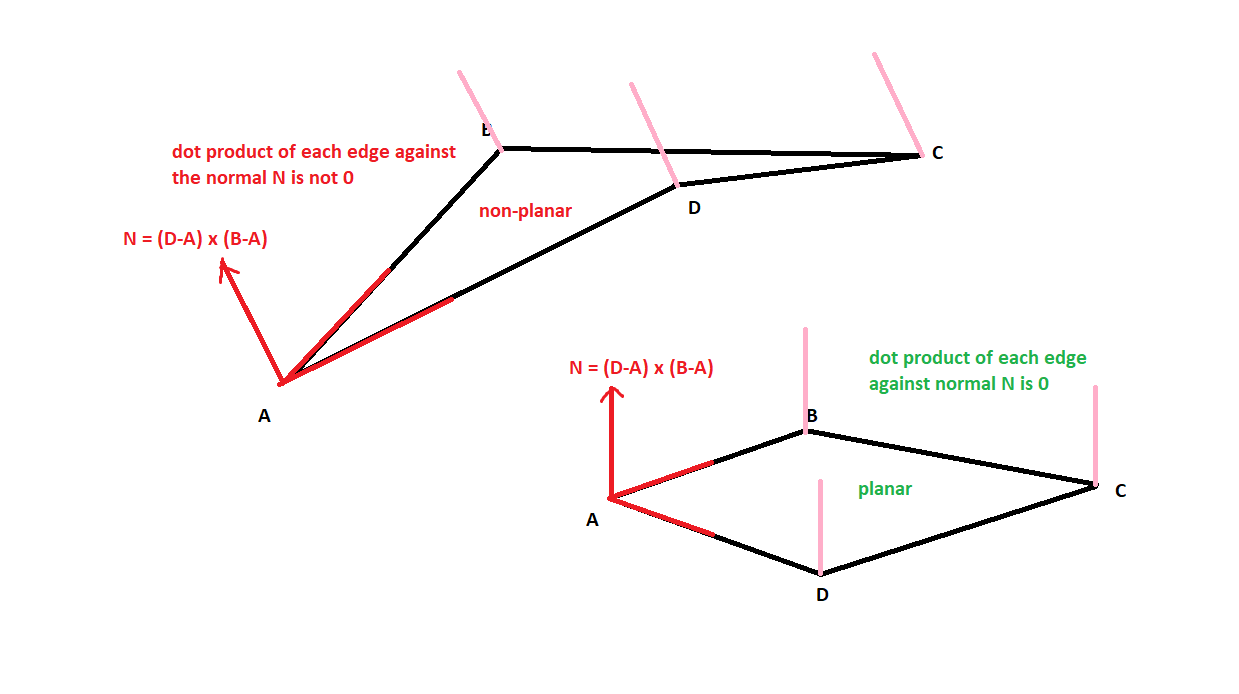
\includegraphics[scale=0.3]{q9-planar.png}

\end{frame}

\section{Question 10}

\begin{frame}
    \frametitle{Question 10}

    Devise a test to check whether a polygon on the x-y plane is convex.
\end{frame}

\begin{frame}
    \frametitle{What is a convex polygon}

    Convex polygon is a polygon that is identical to its \textbf{convex hull}.\\

    \begin{center}
        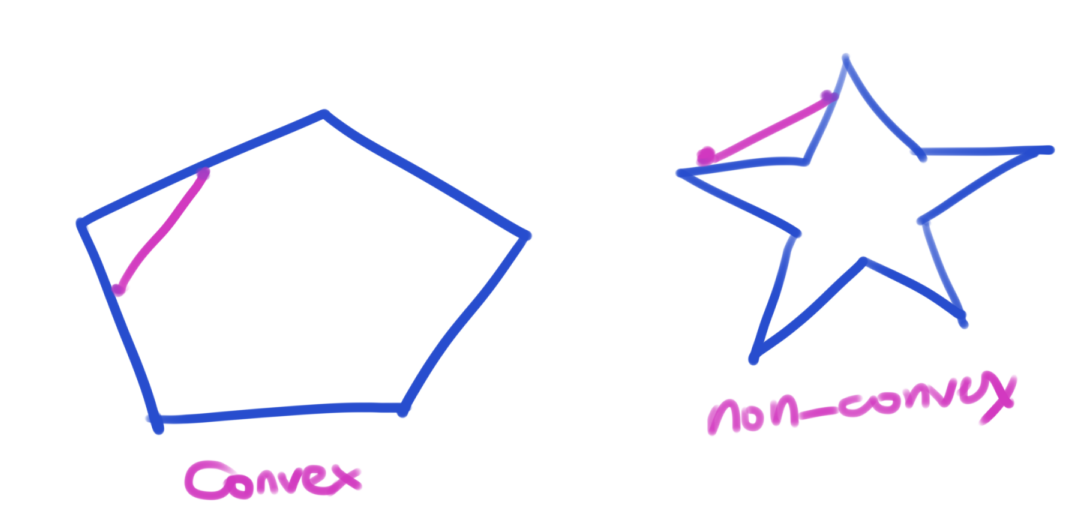
\includegraphics[scale=0.3]{convex-def.png}
    \end{center}

    If you choose any two points on the boundary of a convex polygon and draw a line between, 
    the line should be entirely contained within the polygon.

\end{frame}

\begin{frame}
    \frametitle{Method from Tutorial answer}

    \begin{center}
        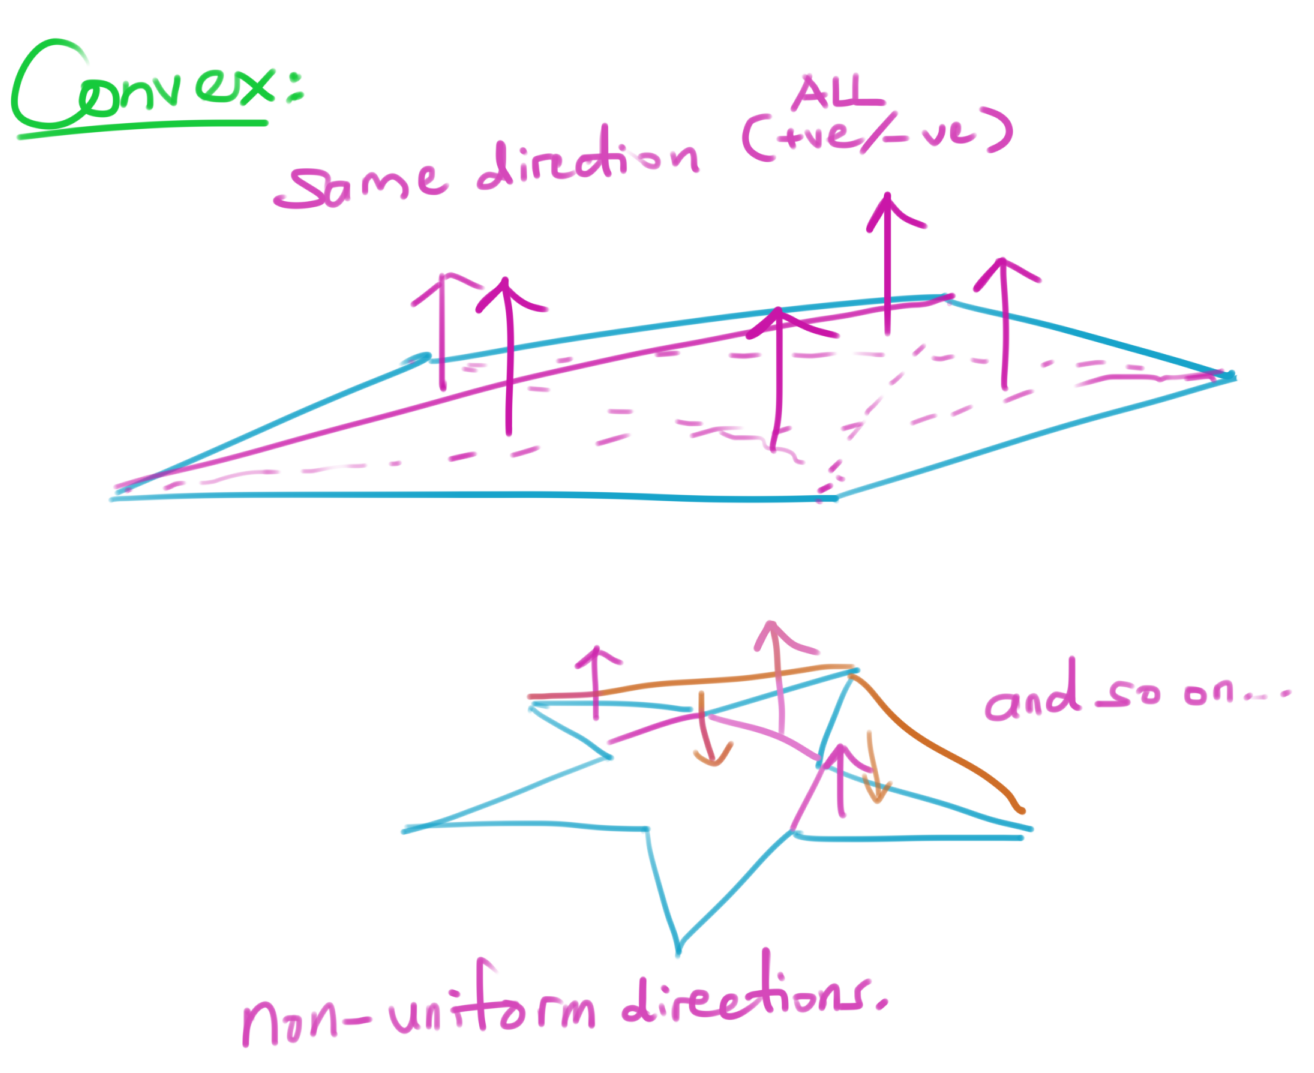
\includegraphics[scale=0.2]{convex.png}
    \end{center}

    Iterating through $i = 0$ to $n-1$ where there are $n$ vertices, find each

    $$
    n_i = \|(v_{i-1} - v_{i}) \times (v_{i+1} - v_{i})\|
    $$
    
    if \textbf{at least one $n_i$ is not identical to the rest}, then polygon is non-convex.

    {\tiny Note: I'm omitting that you have to take the $x\mod n$ of each of the $v_x$ here for conciseness. }
    
\end{frame}

\begin{frame}
    \frametitle{Example of failing convex test}

    $$
    \textcolor{green}{n_i} = \|\textcolor{red}{(v_{i-1} - v_{i})} \times \textcolor{blue}{(v_{i+1} - v_{i})}\|
    $$

    \begin{center}
        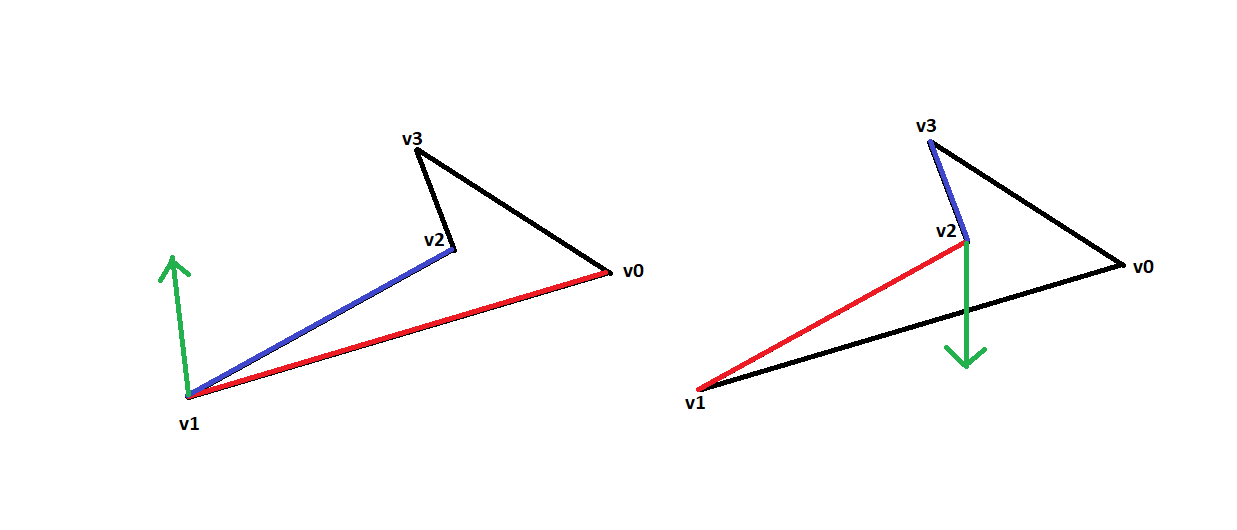
\includegraphics[scale=0.3]{opp-dir.png}
    \end{center}

\end{frame}

\begin{frame}
    \frametitle{Cross product \textbf{Right hand} rule}

    \begin{center}
        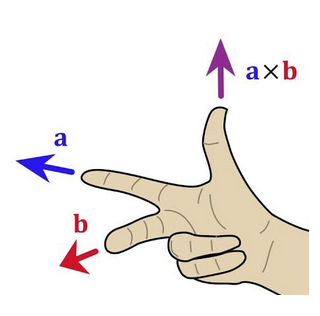
\includegraphics[scale=0.6]{cross-prod.png}
    \end{center}

\end{frame}

\begin{frame}
    \frametitle{What about inner angles?}

    One property of convex polygons: all interior angles $<180^{\circ}$

    \vspace{1em}

    \begin{center}
        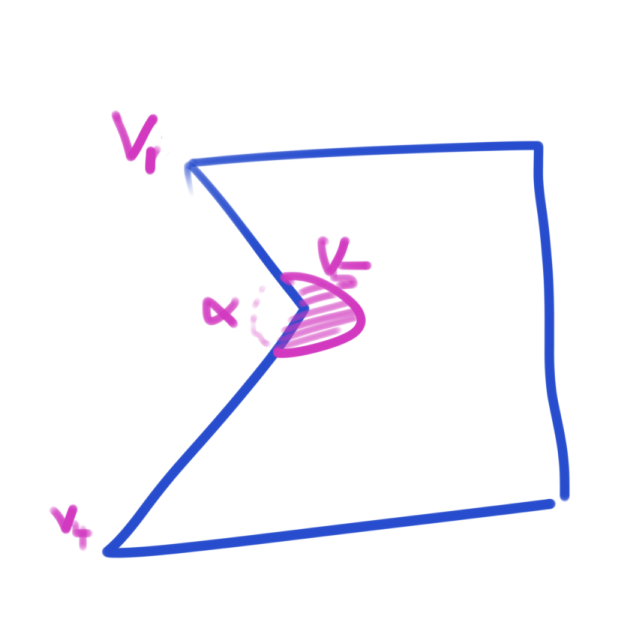
\includegraphics[scale=0.4]{dot-prod.png}
    \end{center}

    Checking this is tricky as the dot product of the vectors $v_4- v_5$ and $v_1 - v_5$ gives you $\cos\alpha$, 
    not the cosine of the interior angle $2\pi - \alpha$.

    One way would be to compute the cross product, which we would have done so using the other method anyway.

\end{frame}


\ThankYou
\begin{frame}[plain,standout]
    Thanks! Get the slides here.\\
    \vspace{2em}
    \scalebox{3}{\faGithub}\par\bigskip
    \url{https://trxe.github.io/cs3241-notes}
\end{frame}

\end{document}